% GNUPLOT: LaTeX picture with Postscript
\begingroup
  \makeatletter
  \providecommand\color[2][]{%
    \GenericError{(gnuplot) \space\space\space\@spaces}{%
      Package color not loaded in conjunction with
      terminal option `colourtext'%
    }{See the gnuplot documentation for explanation.%
    }{Either use 'blacktext' in gnuplot or load the package
      color.sty in LaTeX.}%
    \renewcommand\color[2][]{}%
  }%
  \providecommand\includegraphics[2][]{%
    \GenericError{(gnuplot) \space\space\space\@spaces}{%
      Package graphicx or graphics not loaded%
    }{See the gnuplot documentation for explanation.%
    }{The gnuplot epslatex terminal needs graphicx.sty or graphics.sty.}%
    \renewcommand\includegraphics[2][]{}%
  }%
  \providecommand\rotatebox[2]{#2}%
  \@ifundefined{ifGPcolor}{%
    \newif\ifGPcolor
    \GPcolorfalse
  }{}%
  \@ifundefined{ifGPblacktext}{%
    \newif\ifGPblacktext
    \GPblacktexttrue
  }{}%
  % define a \g@addto@macro without @ in the name:
  \let\gplgaddtomacro\g@addto@macro
  % define empty templates for all commands taking text:
  \gdef\gplbacktext{}%
  \gdef\gplfronttext{}%
  \makeatother
  \ifGPblacktext
    % no textcolor at all
    \def\colorrgb#1{}%
    \def\colorgray#1{}%
  \else
    % gray or color?
    \ifGPcolor
      \def\colorrgb#1{\color[rgb]{#1}}%
      \def\colorgray#1{\color[gray]{#1}}%
      \expandafter\def\csname LTw\endcsname{\color{white}}%
      \expandafter\def\csname LTb\endcsname{\color{black}}%
      \expandafter\def\csname LTa\endcsname{\color{black}}%
      \expandafter\def\csname LT0\endcsname{\color[rgb]{1,0,0}}%
      \expandafter\def\csname LT1\endcsname{\color[rgb]{0,1,0}}%
      \expandafter\def\csname LT2\endcsname{\color[rgb]{0,0,1}}%
      \expandafter\def\csname LT3\endcsname{\color[rgb]{1,0,1}}%
      \expandafter\def\csname LT4\endcsname{\color[rgb]{0,1,1}}%
      \expandafter\def\csname LT5\endcsname{\color[rgb]{1,1,0}}%
      \expandafter\def\csname LT6\endcsname{\color[rgb]{0,0,0}}%
      \expandafter\def\csname LT7\endcsname{\color[rgb]{1,0.3,0}}%
      \expandafter\def\csname LT8\endcsname{\color[rgb]{0.5,0.5,0.5}}%
    \else
      % gray
      \def\colorrgb#1{\color{black}}%
      \def\colorgray#1{\color[gray]{#1}}%
      \expandafter\def\csname LTw\endcsname{\color{white}}%
      \expandafter\def\csname LTb\endcsname{\color{black}}%
      \expandafter\def\csname LTa\endcsname{\color{black}}%
      \expandafter\def\csname LT0\endcsname{\color{black}}%
      \expandafter\def\csname LT1\endcsname{\color{black}}%
      \expandafter\def\csname LT2\endcsname{\color{black}}%
      \expandafter\def\csname LT3\endcsname{\color{black}}%
      \expandafter\def\csname LT4\endcsname{\color{black}}%
      \expandafter\def\csname LT5\endcsname{\color{black}}%
      \expandafter\def\csname LT6\endcsname{\color{black}}%
      \expandafter\def\csname LT7\endcsname{\color{black}}%
      \expandafter\def\csname LT8\endcsname{\color{black}}%
    \fi
  \fi
    \setlength{\unitlength}{0.0500bp}%
    \ifx\gptboxheight\undefined%
      \newlength{\gptboxheight}%
      \newlength{\gptboxwidth}%
      \newsavebox{\gptboxtext}%
    \fi%
    \setlength{\fboxrule}{0.5pt}%
    \setlength{\fboxsep}{1pt}%
\begin{picture}(8496.00,5040.00)%
    \gplgaddtomacro\gplbacktext{%
      \csname LTb\endcsname%
      \put(733,1663){\makebox(0,0){\strut{}$0$}}%
      \put(1376,1582){\makebox(0,0){\strut{}$0.5$}}%
      \put(2020,1501){\makebox(0,0){\strut{}$1$}}%
      \put(2870,1515){\makebox(0,0){\strut{}$-0.5$}}%
      \put(3366,1702){\makebox(0,0){\strut{}$0$}}%
      \put(3861,1888){\makebox(0,0){\strut{}$0.5$}}%
      \put(459,2062){\makebox(0,0)[r]{\strut{}$-0.1$}}%
      \put(459,2536){\makebox(0,0)[r]{\strut{}$0$}}%
      \put(459,3008){\makebox(0,0)[r]{\strut{}$0.1$}}%
      \put(-75,2536){\makebox(0,0){\strut{}z}}%
    }%
    \gplgaddtomacro\gplfronttext{%
      \csname LTb\endcsname%
      \put(1318,1365){\makebox(0,0){\strut{}x}}%
      \put(3753,1507){\makebox(0,0){\strut{}y}}%
      \put(-75,2536){\makebox(0,0){\strut{}z}}%
    }%
    \gplgaddtomacro\gplbacktext{%
      \csname LTb\endcsname%
      \put(4540,1420){\makebox(0,0)[r]{\strut{}$-1$}}%
      \put(4540,1703){\makebox(0,0)[r]{\strut{}$-0.8$}}%
      \put(4540,1985){\makebox(0,0)[r]{\strut{}$-0.6$}}%
      \put(4540,2268){\makebox(0,0)[r]{\strut{}$-0.4$}}%
      \put(4540,2551){\makebox(0,0)[r]{\strut{}$-0.2$}}%
      \put(4540,2834){\makebox(0,0)[r]{\strut{}$0$}}%
      \put(4540,3117){\makebox(0,0)[r]{\strut{}$0.2$}}%
      \put(4540,3399){\makebox(0,0)[r]{\strut{}$0.4$}}%
      \put(4540,3682){\makebox(0,0)[r]{\strut{}$0.6$}}%
      \put(4540,3965){\makebox(0,0)[r]{\strut{}$0.8$}}%
      \put(4672,1129){\makebox(0,0){\strut{}$0$}}%
      \put(5420,1129){\makebox(0,0){\strut{}$2$}}%
      \put(6167,1129){\makebox(0,0){\strut{}$4$}}%
      \put(6915,1129){\makebox(0,0){\strut{}$6$}}%
      \put(7662,1129){\makebox(0,0){\strut{}$8$}}%
      \put(8410,1129){\makebox(0,0){\strut{}$10$}}%
    }%
    \gplgaddtomacro\gplfronttext{%
      \csname LTb\endcsname%
      \put(3968,2657){\rotatebox{-270}{\makebox(0,0){\strut{}energy}}}%
      \put(6541,964){\makebox(0,0){\strut{}time t}}%
      \csname LTb\endcsname%
      \put(7480,3501){\makebox(0,0)[r]{\strut{}Kinetic energy}}%
      \csname LTb\endcsname%
      \put(7480,3281){\makebox(0,0)[r]{\strut{}Potential energy}}%
      \csname LTb\endcsname%
      \put(7480,3061){\makebox(0,0)[r]{\strut{}Total energy}}%
    }%
    \gplbacktext
    \put(0,0){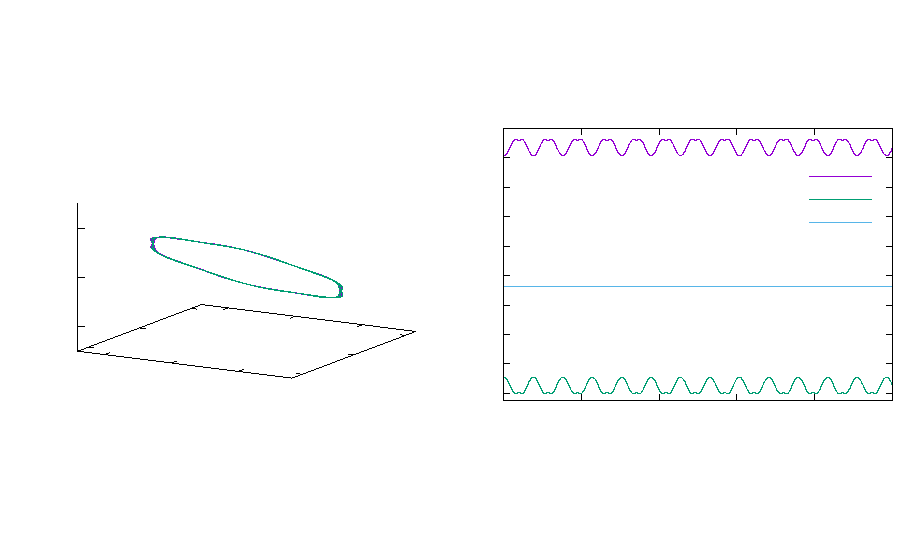
\includegraphics{MDSLP1}}%
    \gplfronttext
  \end{picture}%
\endgroup
